\documentclass[12pt,]{article}
\usepackage{lmodern}
\usepackage{amssymb,amsmath}
\usepackage{ifxetex,ifluatex}
\usepackage{fixltx2e} % provides \textsubscript
\ifnum 0\ifxetex 1\fi\ifluatex 1\fi=0 % if pdftex
  \usepackage[T1]{fontenc}
  \usepackage[utf8]{inputenc}
\else % if luatex or xelatex
  \ifxetex
    \usepackage{mathspec}
  \else
    \usepackage{fontspec}
  \fi
  \defaultfontfeatures{Ligatures=TeX,Scale=MatchLowercase}
\fi
% use upquote if available, for straight quotes in verbatim environments
\IfFileExists{upquote.sty}{\usepackage{upquote}}{}
% use microtype if available
\IfFileExists{microtype.sty}{%
\usepackage{microtype}
\UseMicrotypeSet[protrusion]{basicmath} % disable protrusion for tt fonts
}{}
\usepackage[margin=1in]{geometry}
\usepackage{hyperref}
\hypersetup{unicode=true,
            pdftitle={Researchers collaborate with same-gendered colleagues more often than expected across the life sciences},
            pdfauthor={Luke Holman* and Claire Morandin; *;},
            pdfborder={0 0 0},
            breaklinks=true}
\urlstyle{same}  % don't use monospace font for urls
\usepackage{graphicx,grffile}
\makeatletter
\def\maxwidth{\ifdim\Gin@nat@width>\linewidth\linewidth\else\Gin@nat@width\fi}
\def\maxheight{\ifdim\Gin@nat@height>\textheight\textheight\else\Gin@nat@height\fi}
\makeatother
% Scale images if necessary, so that they will not overflow the page
% margins by default, and it is still possible to overwrite the defaults
% using explicit options in \includegraphics[width, height, ...]{}
\setkeys{Gin}{width=\maxwidth,height=\maxheight,keepaspectratio}
\IfFileExists{parskip.sty}{%
\usepackage{parskip}
}{% else
\setlength{\parindent}{0pt}
\setlength{\parskip}{6pt plus 2pt minus 1pt}
}
\setlength{\emergencystretch}{3em}  % prevent overfull lines
\providecommand{\tightlist}{%
  \setlength{\itemsep}{0pt}\setlength{\parskip}{0pt}}
\setcounter{secnumdepth}{0}
% Redefines (sub)paragraphs to behave more like sections
\ifx\paragraph\undefined\else
\let\oldparagraph\paragraph
\renewcommand{\paragraph}[1]{\oldparagraph{#1}\mbox{}}
\fi
\ifx\subparagraph\undefined\else
\let\oldsubparagraph\subparagraph
\renewcommand{\subparagraph}[1]{\oldsubparagraph{#1}\mbox{}}
\fi

%%% Use protect on footnotes to avoid problems with footnotes in titles
\let\rmarkdownfootnote\footnote%
\def\footnote{\protect\rmarkdownfootnote}

%%% Change title format to be more compact
\usepackage{titling}

% Create subtitle command for use in maketitle
\newcommand{\subtitle}[1]{
  \posttitle{
    \begin{center}\large#1\end{center}
    }
}

\setlength{\droptitle}{-2em}

  \title{Researchers collaborate with same-gendered colleagues more often than
expected across the life sciences}
    \pretitle{\vspace{\droptitle}\centering\huge}
  \posttitle{\par}
    \author{Luke Holman* and Claire Morandin\textsuperscript{§} \\ *\textit{luke.holman@unimelb.edu.au} \\ \textsuperscript{§}\textit{claire.morandin@helsinki.fi} \vspace{5mm}}
    \preauthor{\centering\large\emph}
  \postauthor{\par}
    \date{}
    \predate{}\postdate{}
  
\usepackage{microtype} \usepackage[all]{hypcap} \usepackage{amsmath}
\usepackage{booktabs} \usepackage{caption}
\usepackage[labelfont=bf]{caption} \usepackage{titling}
\pretitle{\begin{flushleft}\LARGE}
\posttitle{\par\end{flushleft}\vskip 0.5em}
\preauthor{\begin{flushleft}\large \lineskip 0.5em}
\postauthor{\par\end{flushleft}} \predate{\begin{flushleft}\large}
\postdate{\par\end{flushleft}} \usepackage{fancyhdr} \pagestyle{fancy}
\fancyhead[LO,LE]{\textsl{\leftmark}} \rhead[]{Gender and coauthorship}
\usepackage[noabbrev,capitalise]{cleveref} \usepackage{titlefoot}
\usepackage{amssymb} \usepackage{rotating} \usepackage{lineno}
\linenumbers

\begin{document}
\maketitle
\begin{abstract}
Evidence suggests that women in academia are hindered by conscious and
unconscious biases, and often feel excluded from formal and informal
opportunities for research collaboration. In addition to ensuring
fairness and helping to redress gender imbalance in the academic
workforce, increasing women's access to collaboration could help
scientific progress by drawing on more of the available human capital.
Here, we test whether researchers tend to collaborate with same-gendered
colleagues, using more stringent methods and a larger dataset than in
past work. Our results reaffirm that researchers co-publish with
colleagues of the same gender more often than expected by chance, and
show that this `gender homophily' is slightly stronger today than it was
10 years ago. Contrary to our expectations, we found no evidence that
homophily is driven mostly by senior academics, and no evidence that
homophily is stronger in fields where women are in the minority.
Interestingly, journals with a high impact factor for their discipline
tended to have comparatively low homophily, as predicted if mixed-gender
teams produce better research. We discuss some potential causes of
gender homophily in science. \vspace{5mm}

\par

\noindent \textbf{Keywords:} Gender bias, Homophily, Research
collaboration, Text mining, Women in STEM.
\end{abstract}

\maketitle\unmarkedfntext{*School of BioSciences, The University of Melbourne, Victoria, Australia.}
\maketitle\unmarkedfntext{\textsuperscript{§}Organismal and Evolutionary Biology Research Programme,
Faculty of Biological and Environmental Sciences, University of Helsinki, Finland.}

\newpage

\hypertarget{introduction}{%
\section{Introduction}\label{introduction}}

Women are severely underrepresented in many branches of science,
technology, engineering, mathematics, and medicine (STEMM), and face
additional challenges and inequities relative to men {[}1--5{]}. On
average, women occupy more junior positions {[}6,7{]} with lower
salaries {[}8,9{]}, receive less grant money {[}10,11{]}, are promoted
more slowly {[}12--15{]}, and are allocated fewer resources {[}16{]} and
less research funding {[}17--19{]}. Experimental evidence suggests that
bias against women plays a major role in generating these differences
{[}20,21{]}.

Writing papers, networking, and collaboration are all instrumental to
research productivity and academic career advancement {[}22--25{]}, and
dozens of studies have tested for gender differences in these areas
{[}5,26--29{]}. For example, studies have concluded that women tend to
be less involved in international collaboration {[}19,28,30--32{]},
collaborate less within their own university departments {[}31{]}, have
less prestigious collaborations {[}33{]}, and fewer collaborations in
total {[}34{]}. These gender differences in collaboration practice
presumably have multiple causes, which might include implicit and
explicit gender bias {[}20{]}, differential family obligations
{[}33,35,36{]}, gender differences in confidence or self-esteem
{[}37{]}, concerns relating to sexual harassment {[}38{]}, and unequal
access to conferences {[}39{]} or travel funds {[}32{]}.

A high, steadily increasing proportion of research papers is written by
more than one author {[}3{]}, making collaboration a key predictor of
publication output, and thus of career prospects {[}40,41{]}.
Additionally, empirical studies imply that mixed-gender or otherwise
diverse teams produce better outputs on collaborative tasks than less
diverse teams {[}42--48{]}. For reasons such as these, multiple studies
have examined the author lists of published research articles in order
to test for gender differences in collaboration frequency or pattern. To
our knowledge, most or all such studies imply that men co-publish with
men, and women with women, more often than expected if collaborators
assort randomly with respect to gender {[}49--58{]}. This pattern of
assortative publishing has often been termed `gender homophily'.

However, we believe that earlier studies of gender homophily were
hindered by a largely unacknowledged statistical issue that we will
refer to as the Wahlund effect (\autoref{wahlund_plot}), by analogy with
the conceptually similar Wahlund effect in population genetics {[}59{]}.
The Wahlund effect makes it deceptively difficult to infer gender-based
preferences simply by counting the number of same- and mixed-gender
coauthorships. Essentially, whenever coauthorship data are sampled from
two or more discrete sets of literature, which vary in the author gender
ratio and which are largely not connected by collaboration, the number
of same-gendered coauthors will be inflated. This can give the
impression that authors preferentially publish with same-gendered
colleagues even if no gender preferences exist, or if the true
preference is for opposite-gendered colleagues (`gender heterophily').
For example, a sample of literature containing a mixture of
bioinformatics and cell biology papers will probably contain an excess
of mostly-male and mostly-female author lists, simply because
researchers usually collaborate within their own discipline, and because
the author gender ratio is more male-biased in bioinformatics than in
cell biology {[}5{]}.

\begin{figure}
\centering
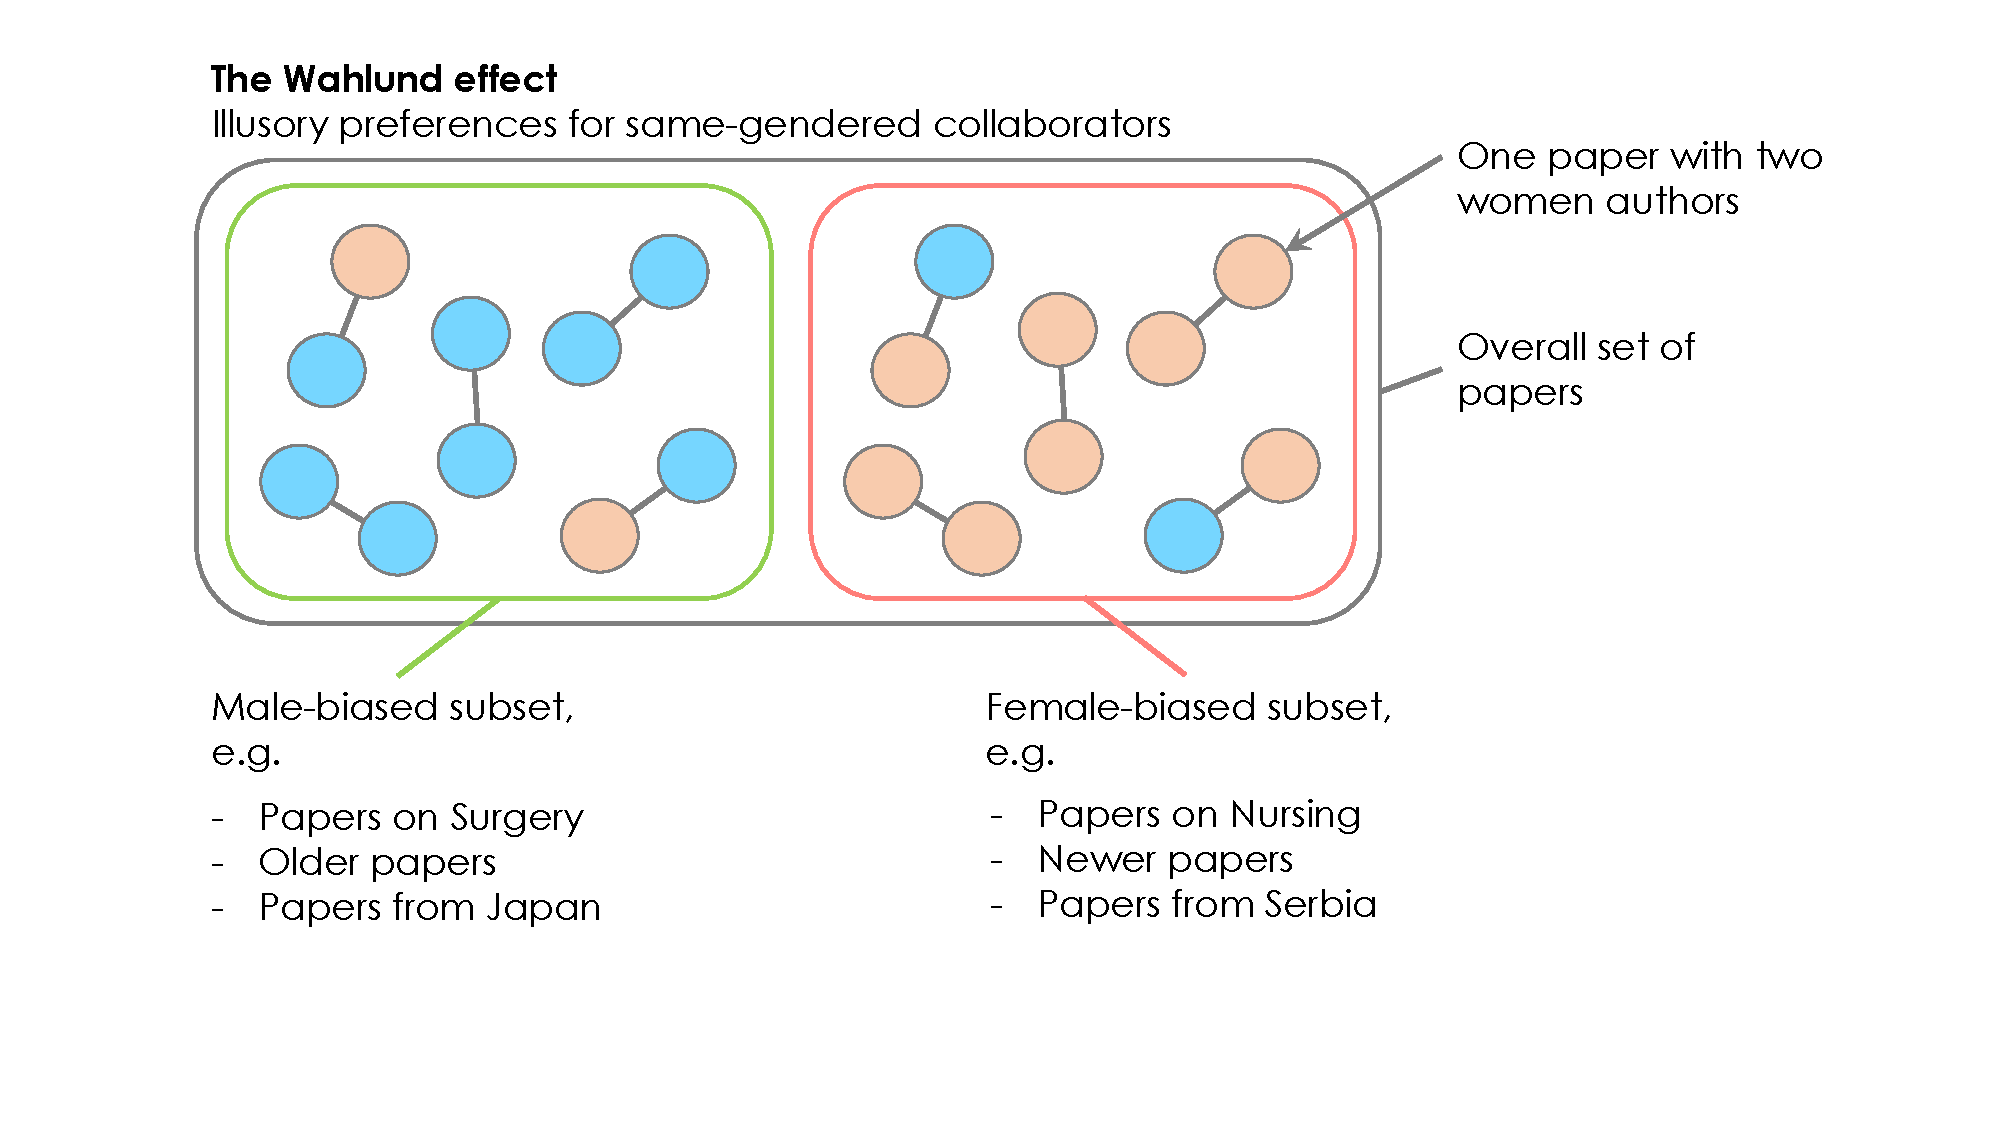
\includegraphics{../figures/Fig1.pdf}
\caption{The Wahlund effect can make it appear as if authors publish
with same-gendered colleagues disproportionately often, even if
collaboration is completely random with respect to gender. Here,
coloured circles represent male and female authors, and coauthors are
linked with lines. Across the whole set of ten papers, there is an
apparent excess of same-gender collaborations: there are six same-gender
papers and only four mixed-gender papers, which is fewer than the
\(10\times2\times0.5\times0.5 = 5\) mixed-gender papers expected under
the null hypothesis that authors assort randomly. However, within each
subset, there is no evidence that authors prefer to publish with
same-gendered individuals (if anything, this small dataset suggests
gender heterophily). The Wahlund effect will tend to inflate the
frequency of same-gender coauthorships whenever the data is composed of
two or more disconnected subsets of literature with different author
gender ratios; these subsets could be research disciplines, older versus
newer papers, or papers from authors in different countries. The example
countries and disciplines were selected based on data in {[}5{]}.
\label{wahlund_plot}}
\end{figure}

In the present study, we test whether life sciences researchers tend to
co-publish with same-gendered colleagues, while controlling for the
Wahlund effect as strictly as possible. We use a recently-published
dataset describing the gender of 35.5 million authors from 9.15 million
articles indexed on PubMed {[}5{]}. Holman et al. {[}5{]} reported large
differences in the gender ratio of authors across research disciplines,
journals, countries, and across the years 2002-2016. We therefore tested
for gender homophily while restricting our analysis to particular
journals (i.e.~research specialties), time periods, and countries. We
quantified gender assortment using a metric called \(\alpha'\) {[}60{]},
which is positive when same-gender authors publish together more often
than expected (gender homophily), negative when opposite-gender authors
publish together more often than expected (heterophily), and equal to
zero when authors assort randomly with respect to gender (see Methods).

\hypertarget{results}{%
\section{Results}\label{results}}

\hypertarget{gender-homophily-by-discipline-time-period-and-authorship-position}{%
\subsection{Gender homophily by discipline, time period, and authorship
position}\label{gender-homophily-by-discipline-time-period-and-authorship-position}}

\autoref{alpha_histograms} shows the distribution of \(\alpha'\)
estimates in 2015-2016 across all journals for which we recovered
sufficient data, when \(\alpha'\) was calculated for all authors, first
authors only, or last authors only. Most journals had positive values of
\(\alpha'\) (77-92\%, depending on time period and author type; S1
Data), and for many of these the false discovery rate (FDR)-corrected
p-values suggested that \(\alpha'\) was significantly greater than zero
(1469/2077 journals were significant in 2015-16, and 404/1192 in 2005-6;
S1 Data). Only 2/2077 journals had statistically significant heterophily
(i.e. \(\alpha' < 0\)) in 2015-16, and 1/1192 in 2005-6 (S2 Table). The
remaining 606 or 787 journals (in 2015 and 2005 respectively) had a
value of \(\alpha'\) not significantly different from zero, consistent
with the null hypothesis of random assortment with respect to gender. We
also confirmed that in most journals (S2 Data) and most research
disciplines (S3 Data, S1 Fig), the majority of papers had multiple
authors.

\begin{figure}
\centering
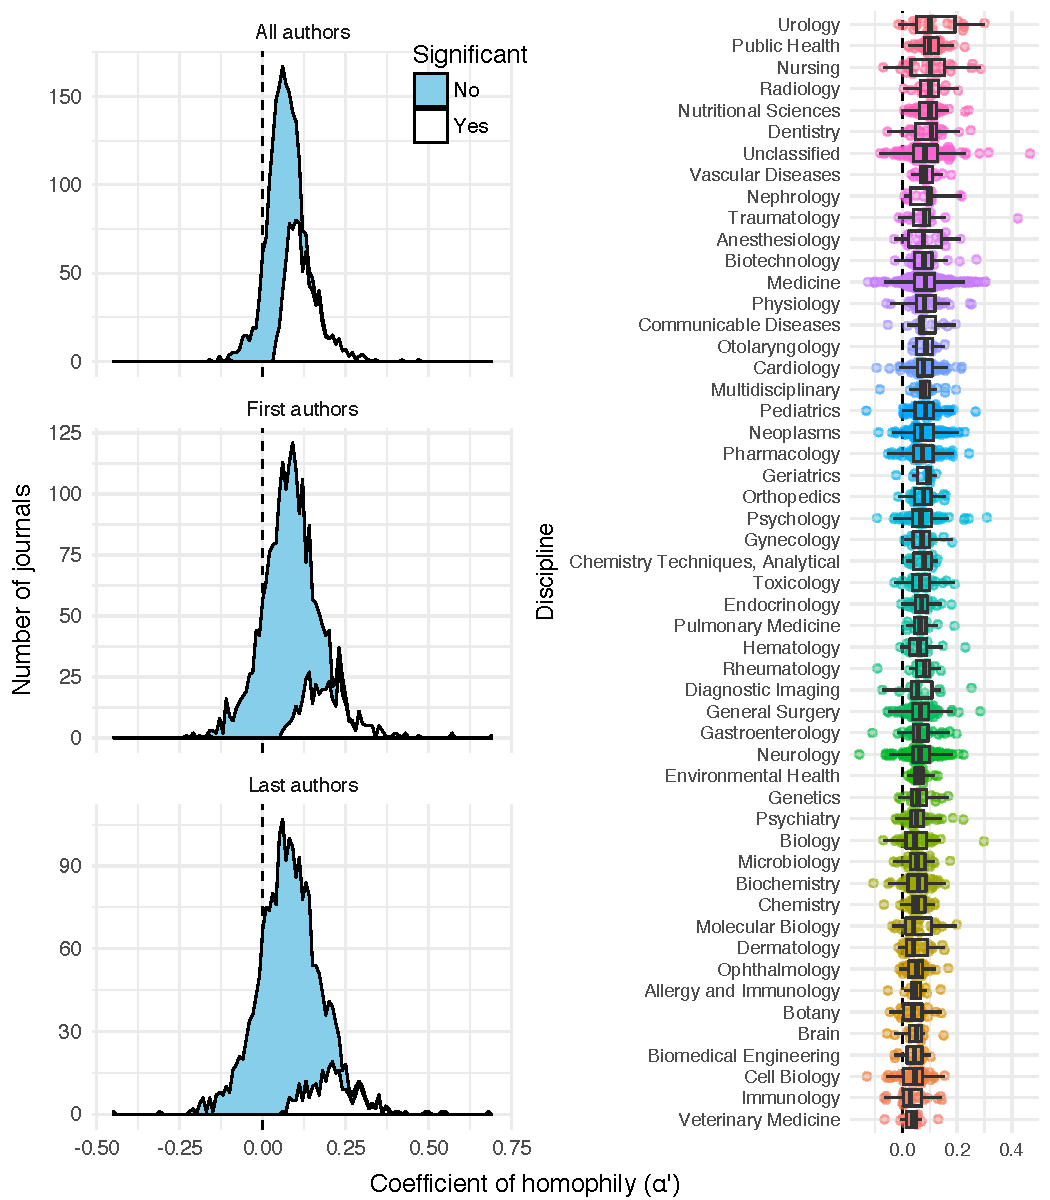
\includegraphics{../figures/Fig2.pdf}
\caption{Of the 2116 journals for which we had adequate data in
2015-2016, 825 showed statistically significant evidence of gender
homophily (denoted by \(\alpha' > 0\)), and 1 showed statistically
significant evidence of heterophily (\(\alpha' < 0\)), after false
discovery rate correction. In the stacked density plot, the white area
shows the number of journals for which homophily was significantly
stronger than expected under the null hypothesis (corrected p
\textless{} 0.05), while the blue area shows all the remainder. Patterns
were similar whether \(\alpha'\) was calculated for all authors, for
first authors only, or for last authors only. Points in the right panel
show \(\alpha'\) for individual journals.\label{alpha_histograms}}
\end{figure}

\(\alpha'\) was significantly higher in the literature sample from
2015-16 relative to 2005-6, though the difference in means was small (S2
Fig; Effect of the fixed factor `Time period' in a linear mixed model of
the data for all author positions: Cohen's \(d\) = \(0.091{\pm}0.04\),
\(t_{953}\) = 2.42, p = 0.016).

When comparing pairs of \(\alpha'\) values estimated for the first and
last authors for the same journals, we found that \(\alpha'\) tended to
be higher for first authors than for last authors (S3 Fig; Effect of the
fixed factor `Authorship position' in a linear mixed model: Cohen's
\(d\) = \(0.065{\pm}0.02\), \(t_{2024}\) = 4.28, p \textless{} 0.0001).
This suggests that the gender of the first author was a slightly
stronger predictor of the remaining authors' genders than the gender of
the last author, i.e.~the opposite of what is predicted if senior
scientists are causally responsible for homophily.

\hypertarget{variance-in-homophily-between-disciplines}{%
\subsection{Variance in homophily between
disciplines}\label{variance-in-homophily-between-disciplines}}

\autoref{alpha_histograms} illustrates the variance in journal homophily
values (\(\alpha'\)) across scientific disciplines. All disciplines had
positive mean \(\alpha'\) (averaged over journals), although homophily
appeared somewhat stronger in some disciplines than others (e.g.~mean
\(\alpha'\) was \(0.12{\pm}0.02\) for Urology journals and
\(0.03{\pm}0.01\) for Veterinary Medicine journals;
\autoref{alpha_histograms}, S4 Data). However, there was no formal
evidence for consistent differences in \(\alpha'\) between disciplines:
the random factor `Discipline' explained around 1\% of the variance in
\(\alpha'\) in the two linear mixed models described in the previous
section (see \autoref{alpha_histograms} and mixed models in Online
Supplementary Material). Thus, whatever processes are responsible for
producing positive \(\alpha'\) values appear to be similarly strong in
all the disciplines we examined.

There was no indication that journals publishing on a wide range of
topics have higher \(\alpha'\) values than more specialised journals,
due to the Wahlund effect. For example, the journal category
`Multidisciplinary' -- which includes journals like \emph{PLOS ONE},
\emph{Nature}, \emph{Science}, and \emph{PNAS} -- did not have markedly
elevated \(\alpha'\) (\autoref{alpha_histograms}). This result suggests
that our estimates of homophily, and estimates from some of the earlier
studies listed in the Introduction, are probably not inflated by the
presence of disparate research topics (with variable author gender
ratios) being published within individual journals.

Nevertheless, when we calculated \(\alpha\) across all non-single-author
papers in our entire 15-year PubMed dataset (as before, excluding papers
where at least one author's gender was unknown; n = \textgreater{}3
million papers, \textgreater{}16 million authors), we found that
\(\alpha\) was 0.126. This figure is almost double the median value of
\(\alpha'\) for individual journals (Figure 2; \(\alpha' = 0.070\) for
`All authors'), suggesting that lumping together papers from different
fields and different time periods can indeed produce spurious evidence
for gender homophily as outlined in Figure 1.

\hypertarget{relationship-between-gender-homophily-and-number-of-authors}{%
\subsection{Relationship between gender homophily and number of
authors}\label{relationship-between-gender-homophily-and-number-of-authors}}

Papers with two authors had significantly lower (but still positive)
\(\alpha'\) values relative to papers with more than two authors, on
average (\autoref{author_number}; statistical results in Online
Supplementary Material). Papers with 3, 4 or \(\ge5\) authors had
essentially identical average \(\alpha'\) values. The variance in
\(\alpha'\) across journals was also a little higher for 2-author papers
compared to the remainder (\autoref{author_number}), though part of this
variance is due to the reduced sample size (in terms of number of
authors) for the 2-author papers. One possible explanation for this
finding is that 2-authors papers might be more likely to have an author
list that is evenly split between career stages (e.g.~a postgraduate
student and their supervisor), increasing the chance that the authors
are mixed gender (see Figure 6). The result also suggests that the
processes responsible for gender homophily are similar in small
(e.g.~3-author) and larger (5+ author) collaborations (and across
disciplines where small versus large collaborations are the norm).

\begin{figure}
\centering
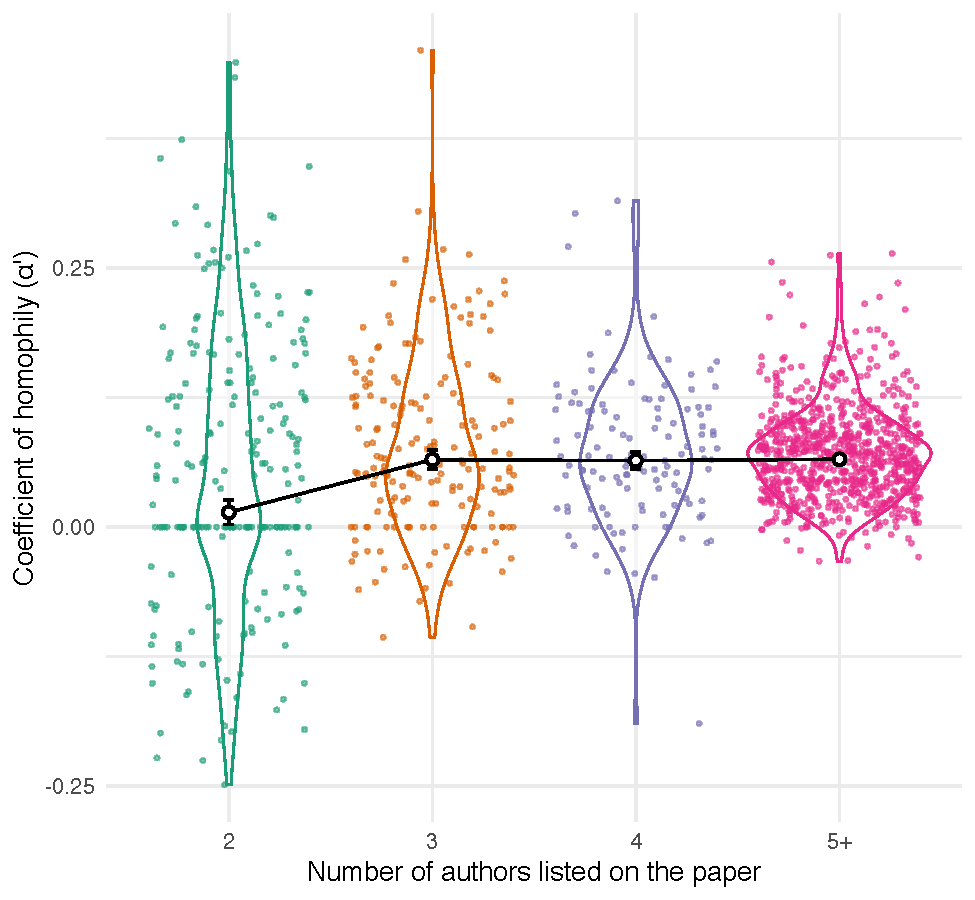
\includegraphics{../figures/Fig3.pdf}
\caption{The coefficient of homophily (\(\alpha'\)) was slightly less
positive when calculated for two-author papers only, relative to papers
with longer author lists. The individual points, whose distribution is
summarised by the violin plots, correspond to individual journals. The
larger white points show the mean for each group (and its 95\% CIs), as
calculated by a Bayesian meta-regression model accounting for repeated
measures of \(\alpha'\) within journals, as well as the precision with
which \(\alpha'\) was estimated. \label{author_number}}
\end{figure}

\hypertarget{relationship-between-gender-homophily-and-gender-ratio}{%
\subsection{Relationship between gender homophily and gender
ratio}\label{relationship-between-gender-homophily-and-gender-ratio}}

We next tested whether researchers are more or less likely to publish
with same-gendered colleagues in strongly gender-biased disciplines
(e.g.~Surgery or Nursing), relative to disciplines with a comparatively
gender-balanced workforce (e.g.~Psychiatry). We found a positive,
non-linear relationship between the overall gender ratio of all authors
publishing in a particular journal {[}5{]}, and the estimated value of
\(\alpha'\) for all authors and for first authors
(\autoref{alpha_gender_ratio}). Journals with a balanced or
female-biased author gender ratio tended to have higher \(\alpha'\)
(i.e.~stronger homophily) than journals with a male-biased author gender
ratio (GAM smooth terms p \textless{} 0.001; Online Supplementary
Material). The relationship was not statistically significant when
\(\alpha'\) was calculated for last authors (GAM, p = 0.142), though the
trend appeared similar (\autoref{alpha_gender_ratio}).

\begin{figure}
\centering
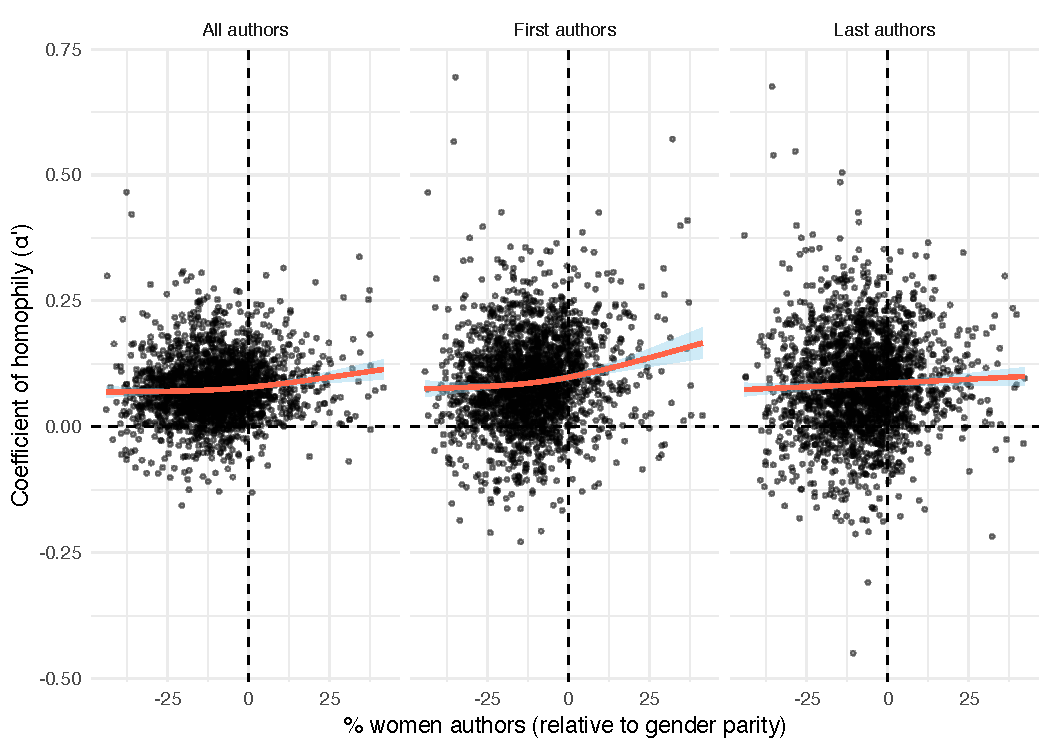
\includegraphics{../figures/Fig4.pdf}
\caption{There is a weakly positive, non-linear relationship between the
gender ratio of authors publishing in a journal, and the coefficient of
homophily (\(\alpha'\)). Specifically, journals with 50\% women authors
or higher tended to have more same-sex coauthorships than did journals
with predominantly men authors. This relationship held whether
\(\alpha'\) was calculated for all authors, first authors only, or last
authors only. A negative value on the x-axis denotes an excess of men
authors, a positive value denotes an excess of women authors, and zero
denotes gender parity (i.e.~equal numbers of men and women). The lines
were fitted using generalised additive models with the smoothing
parameter \(k\) set to 3. \label{alpha_gender_ratio}}
\end{figure}

\hypertarget{relationship-between-journal-impact-factor-and-gender-homophily}{%
\subsection{Relationship between journal impact factor and gender
homophily}\label{relationship-between-journal-impact-factor-and-gender-homophily}}

We observed a noisy but statistically significant linear relationship
between standardised journal impact factor and \(\alpha'\), such that
journals with a high impact factor for their discipline had weaker
gender homophily than did journals with a low impact factor for their
discipline (\autoref{impact_factor}; linear regression: \(R^2\) = 0.043,
\(t_{1415}\) = -8.0, p \textless{} 0.0001). The slope of the regression
was \(-0.012{\pm}0.0015\), indicating that increasing the
discipline-standardised impact factor by one standard deviation is
associated with a reduction in \(\alpha'\) of 0.012.

\begin{figure}
\centering
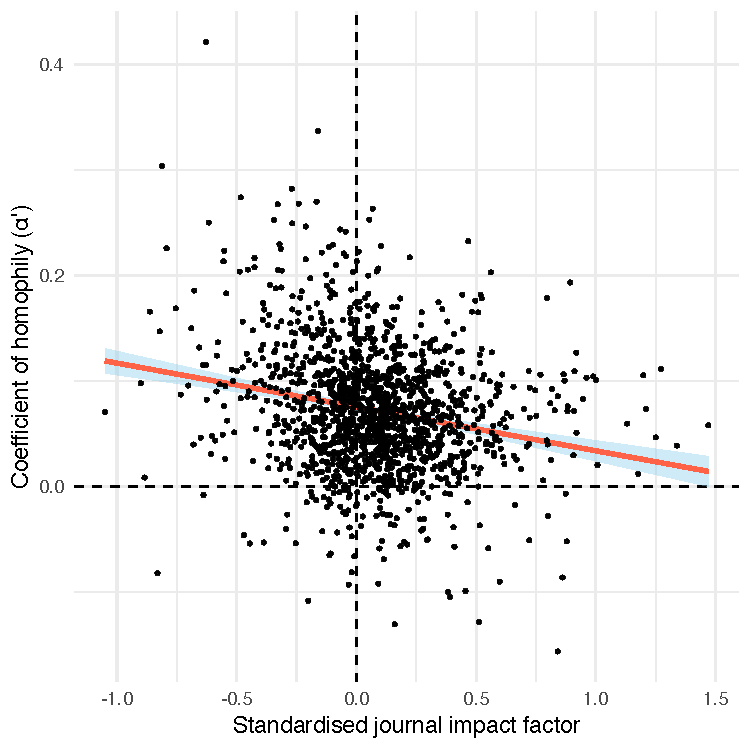
\includegraphics{../figures/Fig5.pdf}
\caption{Journal impact factor (expressed relative to the average for
the discipline) is negatively correlated with \(\alpha'\). The
relationship is noisy (\(R^2\) = 0.043), but the results suggest that
journals with strong homophily tend to have lower impact factors than
journals with weak homophily in the same discipline.
\label{impact_factor}}
\end{figure}

\hypertarget{analysis-accounting-for-differences-in-author-gender-ratio-between-countries}{%
\subsection{Analysis accounting for differences in author gender ratio
between
countries}\label{analysis-accounting-for-differences-in-author-gender-ratio-between-countries}}

When we restricted the analysis by country, we observed statistically
significant homophily for 72 of the 325 journal-country combinations
tested (64 unique journals and 18 unique countries), and no significant
heterophily (S4-S5 Fig). Additionally, the values of \(\alpha'\)
calculated for each journal-country combination were only very slightly
lower than the \(\alpha'\) values calculated for the journal as a whole
(i.e.~when pooling papers from different countries, as was done to make
\autoref{alpha_histograms}): on average, the difference in \(\alpha'\)
was only 0.002 (S6 Fig). These results suggest that our findings of
widespread homophily in the main analysis were not driven solely by a
Wahlund effect resulting from gender differences between countries.

\hypertarget{theoretical-expectations-for-alpha-when-the-gender-ratio-differs-between-career-stages}{%
\subsection{\texorpdfstring{Theoretical expectations for \(\alpha\) when
the gender ratio differs between career
stages}{Theoretical expectations for \textbackslash{}alpha when the gender ratio differs between career stages}}\label{theoretical-expectations-for-alpha-when-the-gender-ratio-differs-between-career-stages}}

Given that we cannot identify individual researchers or their career
stages, we used a simple model to derive the theoretical expectations
for \(\alpha\) when the gender ratio differs between career stages (see
Methods). As shown in \autoref{simulation}, we predict that \(\alpha\)
is expected to be non-zero, even if collaborators are randomly selected
with respect to gender, provided that there is a gender gap between
career stages. The extent to which \(\alpha\) deviates from zero depends
on the relative frequencies of collaboration within and between career
stages (rows and columns in Figure 6), and the size of the gender gap
between stages (x- and y-axes in Figure 6). When \textgreater{}50\% of
coauthor pairs comprise one early-career and one established researcher,
we expect gender heterophily (\(\alpha < 0\)) whenever the gender ratio
differs between career stages. Conversely, when \textgreater{}50\% of
collaborations are between people at the same career stage, we expect
gender homophily (\(\alpha > 0\)). In a few parameter spaces (shown in
red; \autoref{simulation}), \(\alpha\) was quite high, and overlapped
with the values that we estimated (\autoref{alpha_histograms}).

\begin{figure}
\centering
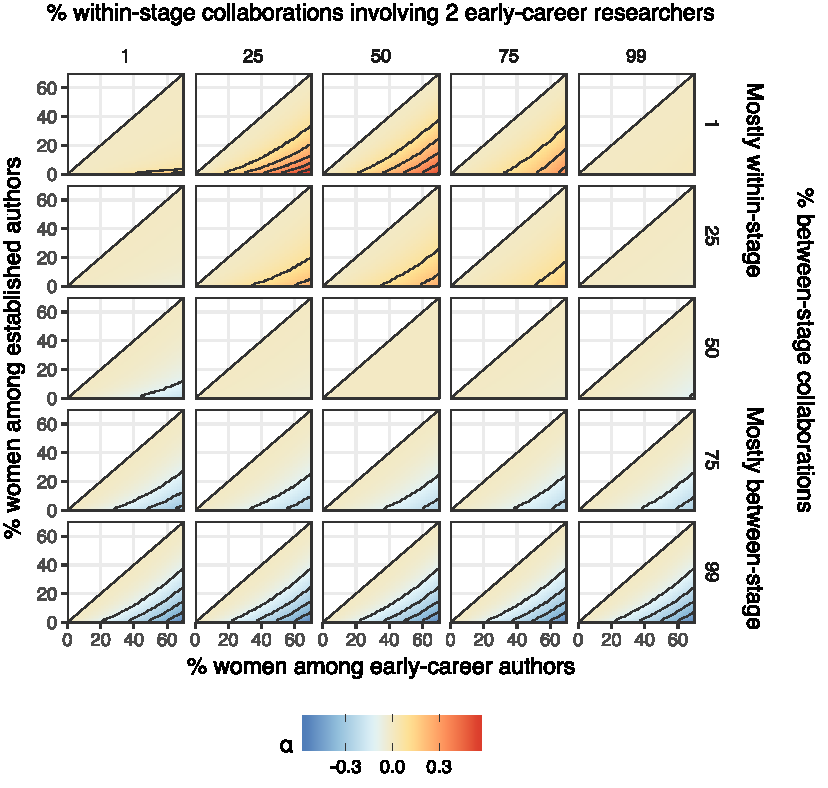
\includegraphics{../figures/Fig6_inkscape.pdf}
\caption{When the gender ratio of early-career researchers is not equal
to the gender ratio among established researchers, the null expectation
for \(\alpha\) is not necessarily zero. Specifically, if most
collaborations occur between career stages, there will be an excess of
mixed-gender collaborations (\(\alpha < 0\), blue areas), while if most
collaborator pairs comprise two people at the same career stage, there
will be an excess of same-gender collaborations (\(\alpha > 0\), red
areas). However, the conditions required for strong gender homophily
(i.e.~the red areas) are quite restrictive, making it unlikely that this
issue can fully explain the homophily observed in our study.
Additionally, in research disciplines where between-career stage
collaboration is common and there is a shortage of women among
established researchers (i.e.~the blue areas), our study will
underestimate the strength of gender homophily. Contour lines denote
increments of 0.1. \label{simulation}}
\end{figure}

Despite this overlap, \autoref{simulation} suggests that our main
conclusions (and those of other studies of gender homophily) are
probably robust to this career stage issue. We only expect strongly
positive \(\alpha\) when A) the gender ratio is highly skewed across
career stages (e.g.~a 5-fold difference), and B) collaborations between
early and established researchers are very rare (e.g. \textless{}10\% of
the total). Both of these conditions seem unlikely to be true for most
fields: the gender gap across careers stages is generally less
pronounced {[}1,5{]}, and it is very common for early-career researchers
to co-publish with an established mentor {[}61{]}. However, one can get
\(\alpha > 0\) for realistic combinations of parameters, e.g.~a moderate
shortage of women in senior positions coupled with a moderate excess of
within-career stage collaboration, suggesting this effect might
contribute to some of the homophily observed by this and previous
studies.

Lastly, we note that if there is a gender gap between career stages and
coauthorships between early-career and established researchers comprise
\textgreater{}50\% of the total, then the baseline expectation for
\(\alpha\) is actually less than zero (blue areas in
\autoref{simulation}). Therefore, it is possible that researchers
preferentially assort with same-gendered collaborators even more
strongly than implied by our results, at least for certain journals or
research disciplines.

\hypertarget{discussion}{%
\section{Discussion}\label{discussion}}

We found evidence that researchers work with same-gendered coauthors
more often than expected under the null model, even after implementing
stringent controls for Wahlund effects (\autoref{wahlund_plot}). Our
study therefore reaffirms earlier studies' conclusions {[}49--57,62{]}
using stricter methodology, and generalises their results across the
life sciences. Relatively few journals had \(\alpha'\) values below
zero, and almost no journals showed statistically significant gender
heterophily after controlling for multiple testing. The excess of
same-gender coauthorships was quite large: many journals had
\(\alpha' > 0.1\), indicating that the gender ratio of men's and women's
coauthors differs by \textgreater{}10\% in absolute terms. In relative
terms, our findings are even more striking: for example, if men have
20\% female coauthors and women have 30\% (i.e. \(\alpha' = 0.1\) in a
field with a typical gender ratio {[}5{]}), then women publish with
women 50\% more often than men do.

An important limitation of our study is that we cannot reliably
determine the cause(s) of the observed excess of same-gender
coauthorships. As well as the obvious interpretation -- conscious or
unconscious selection of same-gender collaborators by men, by women, or
both -- our results could be partly explained by uncontrolled Wahlund
effects. However, we suspect the contribution of these uncontrolled
artefacts to be minor, for four reasons: we found positive \(\alpha'\)
after controlling for three obvious sources of Wahlund effect; there was
no inflation of \(\alpha'\) in highly multidisciplinary journals
relative to specialised journals; restricting the data by country
yielded similar estimates of \(\alpha'\); and we used a simple model to
show that differences in gender ratio between career stages are unlikely
to fully explain our results. On balance, we believe the data suggest
that it is likely that some researchers preferentially select
same-gendered collaborators, although it is difficult to ascertain what
proportion of people show such a preference, or how much the strength of
the preference varies between individuals. We also note that even in a
world in which collaboration was completely random with respect to
gender, a high proportion of individual researchers would have entirely
same-gendered collaborators by chance alone (especially in gender-biased
disciplines); thus, individuals who only have same-gendered co-authors
are not necessarily doing anything differently from people with
gender-balanced co-authors.

We hypothesised that disciplines with a strongly skewed gender ratio
might show the strongest gender homophily, e.g.~because being in the
minority might increase people's motivation to seek out same-gendered
colleagues. Contrary to this hypothesis, we found no evidence that
gender homophily is restricted to particular disciplines: \(\alpha'\)
was similarly high across the board (\autoref{alpha_histograms}).
Interestingly, gender homophily was weakest for journals with a
male-biased author gender ratio, and strongest in journals with a
female-biased author gender ratio. One possible reason is that men are
more likely to preferentially seek out male collaborators in fields
where men are a minority, relative to the homophily displayed by women
in fields where women are a minority. However, this latter result only
has tentative statistical support since our sample contains few journals
in which most authors are women (\autoref{alpha_gender_ratio}).

We also found that gender homophily was marginally stronger in 2015-2016
relative to 2005-2006. Although this trend might reflect a change in the
gender preferences of researchers seeking collaborators, there are
alternative (and perhaps more likely) explanations. For example, this
trend might result from the increasing number of women working in senior
positions in STEMM over the past decade {[}63--65{]}. As shown in
\autoref{simulation}, if enough coauthorships are between junior and
senior researchers, a large gender gap between career stages can give
the appearance of heterophily. As this gender gap between career stages
lessens, the observed values of \(\alpha'\) may increase.

Regarding our finding of weaker homophily among 2-author papers, we
suspect that many 2-author teams comprise a student/postdoc and a senior
staff member, making these teams especially likely to be mixed-gender,
due to the greater shortage of women among senior researchers {[}1,5{]}.
Assuming this interpretation is correct, this result suggests that our
reported \(\alpha'\) values may underestimate the strength of peoples'
preferences for same-gendered collaborators; essentially, women seeking
a senior collaborator could be constrained to work mostly with men,
meaning that people's ideal and realised gender preferences would be
mismatched. On a related note, Ghiasi et al. {[}51{]} argue that women
in engineering are ``compliant {[}in reproducing{]} male-dominated
scientific structures'' because they do not collaborate often enough
with other women (for reference, Figure 7 in {[}51{]} implies that
coauthorships involving two women are \(c\). 30\% more frequent than
expected under random assortment). By contrast, we feel that it may be
counter-productive to recommend that women collaborate primarily with
other women, e.g.~because this constrains women's options (particularly
in fields like engineering, where 90\% of professors are men {[}1{]}).
Instead, we suggest that researchers of both genders can help to close
the gender gap in STEMM. In the context of collaboration, one way to do
this is to undertake self-examination to ensure that one is not
inadvertently overlooking or excluding women among potential students
and colleagues. One should also take care to treat male and female
collaborators equally, e.g.~in terms of training and mentoring,
allocation of work, how one frames or promotes the collaboration
(e.g.~in conference presentations or on a website), and in terms of the
credit afforded to collaborators' contributions. Experimental work
suggests that unconscious bias causes people to undervalue women's
research achievements {[}20{]}, and a study of author contribution
statements found observational evidence that menial or under-valued
tasks are assigned to women while more prestigious tasks are assigned to
men {[}61{]}.

Our study begs two questions: what causes gender homophily in science,
and are our results cause for concern? We believe that the answers to
these questions are closely related. For example, some of the homophily
we observed might be caused by women seeking to avoid harassment or
sexism from men {[}38{]}, which would clearly be concerning.
Additionally, Sheltzer and Smith {[}66{]} concluded that `elite' male
academics (defined as recipients of major honours) have a higher
proportion of male students and postdocs than non-elite male academics.
This finding could contribute to the homophily we observed, and is cause
for concern since the results might reflect discrimination against women
during hiring {[}20{]}, or avoidance by women of elite research groups
(e.g.~due to gender differences in confidence, or a perception that some
groups are sexist). We also found a little evidence that gender
homophily is detrimental to research quality, in that high-impact
journals tended to have weaker homophily. Assuming that papers published
in high-impact journals are of higher average quality (which is
contentious; {[}67{]}), our results provide non-experimental support for
the hypothesis that mixed-gender teams produce better research than
single-gender teams {[}42--48{]}. Another issue is that if many
collaborations are between established researchers, there will be an
excess of male-male collaborations in fields where women in senior
positions are rare; some of the observed homophily might therefore
reflect the elevated gender gap among senior researchers.

On the other hand, homophily might have more benign causes.
Collaboration is often most enjoyable and productive when working with
like-minded people, who might tend to be same-gendered more often than
not. We also suppose that some people consciously choose to
preferentially collaborate with women in order to help close the gender
gap in the workforce; this would create homophily if women do this more
than men. In support of this interpretation, there is some evidence that
women are more likely than men to promote the work of female colleagues
by inviting them to give talks {[}68,69{]}. Given that many
collaborative research projects unfortunately involve a gendered
division of labour {[}61{]}, working with a same-gendered colleague may
provide exposure to new parts of the research process, and (especially
for the minority gender) a welcome change of pace.

\hypertarget{methods}{%
\section{Methods}\label{methods}}

\hypertarget{the-dataset}{%
\subsection{The dataset}\label{the-dataset}}

We used the dataset of PubMed author lists from Holman et al. {[}5{]}.
Briefly, that dataset was created by downloading every article indexed
on PubMed and attempting to infer each author's gender from their given
name using computational methods. Each journal was assigned to one of
107 scientific disciplines, using PubMed's journal categorisations in
the interests of objectivity. Because the present study focuses on
co-authorship, all single-author papers were discarded. We also
discarded all papers for which we could not determine the gender of
every author with \({\ge}95\%\) certainty, in order to simplify the
statistical analysis. To mitigate Wahlund effects caused by variation in
the gender ratio of researchers over time (see below), we only kept
papers with publication dates falling in two one-year time periods,
namely 0-1 or 10-11 years prior to the collection date of the PubMed
data (i.e.~20\textsuperscript{th} August 2016). Lastly, we excluded
journals with fewer than 50 suitable papers. Detailed sample size
information is given in S1 Table.

\hypertarget{calculating-alpha-the-coefficient-of-homophily}{%
\subsection{\texorpdfstring{Calculating \(\alpha\), the coefficient of
homophily}{Calculating \textbackslash{}alpha, the coefficient of homophily}}\label{calculating-alpha-the-coefficient-of-homophily}}

Following Bergstrom et al. {[}60{]}, we defined the coefficient of
homophily as \(\alpha = p - q\), where \(p\) is the probability that a
randomly-chosen co-author of a \emph{male} author is a man and \(q\) is
the probability that a randomly-chosen co-author of a \emph{female}
author is a man. Like the Wahlund effect, \(\alpha\) is borrowed from
population genetics; for a set of 2-author papers, it is equivalent to
Wright's coefficient of inbreeding {[}70{]}. Mathematical work
illustrates that \(\alpha\) is closely related to alternative
network-based methods for quantifying homophily {[}71{]}.

To estimate \(\alpha\) for a particular subset of the scientific
literature, we estimated \(p\) as the average proportion of men's
co-authors who are men (averaged across all papers with at least one man
author), and \(q\) as the average proportion of women's co-authors who
are men (averaged across all papers with at least one woman author). To
estimate the 95\% confidence intervals on \(\alpha\) for a given set of
\(n\) papers, we sampled \(n\) papers with replacement 1000 times,
estimated \(\alpha\) on each sample, and recorded the 95\% quantiles of
the resulting 1000 estimates.

As well as calculating \(\alpha\) for all authors, we calculated
\(\alpha\) for first or last authors only. \(\alpha\) was again defined
as \(p - q\), but this time \(p\) was estimated as the average
proportion of male co-authors on papers with a male first (or last)
author, and \(q\) was estimated as the average proportion of male
co-authors on papers with female first (or last) authors. We did not
calculate \(\alpha\) for other authorship positions (e.g.~second or
third authors) because this would necessitate culling the dataset to
include only papers with a sufficiently long author list, complicating
interpretation of the results.

We also calculated \(\alpha\) for papers with 2, 3, 4 or \({\ge}5\)
authors, for all journals that had at least 50 suitable papers from
2015-2016 with the specified author list length.

Our test assumes that the expected value of \(\alpha\) is zero if
authors randomly assort, but for small datasets this assumption is not
always true. Essentially, this issue arises because a person cannot be
their own co-author. In a small dataset comprising \(m\) men and \(f\)
women, a man can co-author with \(m - 1\) men while women can co-author
with \(m\) men. Thus, the null expectation for \(\alpha\) is a negative
number -- potentially a large one if \(m\) and \(f\) are very small.

To control for the fact that the null expectation for \(\alpha\) is not
zero for small datasets, we devised an adjusted version of the
coefficient of homophily, which we term \(\alpha'\). Every time we
calculated \(\alpha\) for a set of papers, we also determined the
expected value of \(\alpha\) under the null hypothesis that authors
assort randomly with respect to gender. This was accomplished by
randomly permuting authors across papers 1000 times, recalculating
\(\alpha\), and taking the median. We then calculated \(\alpha'\) by
subtracting the null expectation for \(\alpha\) from the observed value.
We also used the null-simulated \(\alpha\) values to calculate a
two-tailed p-value for the observed value of \(\alpha\); the p-value was
defined as the proportion of null simulations for which
\(|\alpha_{null}| > |\alpha_{obs}|\). We applied false discovery rate
(FDR) correction to each set of p-values to account for multiple testing
{[}72{]}.

As expected, \(\alpha'\) was usually almost identical to \(\alpha\) (S7
Fig), but \(\alpha\) was downwardly biased relative to \(\alpha'\) for
small datasets (S8 Fig). Additionally, the correlation between
\(\alpha'\) and sample size was negligible (\(R^2 < 0.01\)), suggesting
that our calculation of \(\alpha'\) effectively removed the dependence
of \(\alpha\) on sample size. We therefore used \(\alpha'\) in all
analyses.

\hypertarget{minimising-the-wahlund-effect-research-discipline-and-time-period}{%
\subsection{Minimising the Wahlund effect: research discipline and time
period}\label{minimising-the-wahlund-effect-research-discipline-and-time-period}}

To minimise bias in \(\alpha'\) due to the Wahlund effect, we restricted
each set of papers to a single research specialty to the greatest extent
allowed by our data. Specifically, we only calculated \(\alpha'\) for
individual journals, since papers from the same journal typically focus
on closely related topics. Although some journals, e.g. \emph{PLOS ONE},
publish research from diverse disciplines with very different author
gender ratios {[}5{]}, calculating \(\alpha'\) for these highly
multidisciplinary journals is still useful as a contrast. The difference
in \(\alpha'\) between highly multidisciplinary and more specialised
journals, e.g. \emph{PLOS ONE} versus \emph{PLOS Computational Biology},
gives an estimate of the extent to which multidisciplinarity within
journals inflates \(\alpha'\).

As well as varying between disciplines, the gender ratio of authors has
changed markedly over time {[}5{]}. Because the gender ratio was more
male-biased in the past, \(\alpha'\) would be inflated if we calculated
it for a sample of papers published over a long enough time frame. To
minimise this effect, we only sampled papers from two one-year periods
(namely 2005-6 and 2015-16). The median change per year in \% (fe)male
authors across journals is below 0.5\% {[}5{]}, and so restricting our
dataset to a single year should prevent temporal changes in gender ratio
from noticeably affecting our estimates of \(\alpha'\).

\hypertarget{minimising-the-wahlund-effect-author-country-of-affiliation}{%
\subsection{Minimising the Wahlund effect: author country of
affiliation}\label{minimising-the-wahlund-effect-author-country-of-affiliation}}

A Wahlund effect could arise even if one calculates \(\alpha'\) for a
single discipline and time period, because of variation in the gender
ratio of researchers from different countries. For example, Holman et
al. {[}5{]} found that PubMed-indexed authors based in Serbia are more
than twice as likely to be women as are authors based in Japan.
Therefore, a dataset containing a mix of papers from teams of authors
based in these two countries would contain an excess of same-sex
coauthorships, even if collaboration were random with respect to gender
within each country.

To address this issue, we also analysed every combination of journal and
author country of affiliation for which we had enough data (i.e.~50 or
more papers published in 2015-16). For simplicity, we restricted the
dataset to only include papers for which Holman et al. {[}5{]} had
identified the country of affiliation for all authors on the paper, and
all authors shared the same country of affiliation. Restricting the
dataset in this fashion produced enough data to measure \(\alpha'\) for
325 combinations of journal and country (median: 70 papers and 273
authors per combination).

\hypertarget{calculating-standardised-journal-impact-factor}{%
\subsection{Calculating standardised journal impact
factor}\label{calculating-standardised-journal-impact-factor}}

We obtained the 3-year impact factor for each journal from Clarivate
Analytics (formerly ISI). To account for large differences in impact
factor between disciplines, we took the the residuals from a model with
\(log_{10}\) impact factor as the response and the research discipline
of the journal as a random effect. Thus, journals with a positive
standardised impact factor have a higher mean number of citations than
the average for journals in their discipline. We then used Spearman rank
correlation to test whether \(\alpha'\) was correlated with impact
factor across journals.

\hypertarget{statistical-analysis}{%
\subsection{Statistical analysis}\label{statistical-analysis}}

Previous authors {[}66,73{]} have hypothesised that senior scientists
preferentially recruit staff and students of the same gender, and/or
that junior researchers preferentially select same-gendered mentors. In
the majority of PubMed-indexed disciplines, authorship conventions mean
that the first-listed author is often an early-career researcher, while
the author listed last is more likely to be a senior researcher leading
a research team {[}74{]}. Assuming that senior researchers are the main
drivers of homophily and that there are enough papers with three or more
authors, we predict that the last author's gender will be the strongest
predictor of the remaining authors' genders (i.e.~the gender of the last
author will be more salient than that of the first author, or any other
authorship position). This is because the first author's gender would
simply be an imperfect correlate of the true causal effect, while the
last author's gender would be the causal effect itself.

To test whether \(\alpha'\) for last authors tends to be higher than
\(\alpha'\) for first authors for any given dataset, we used a linear
mixed model implemented in the \texttt{lme4} and \texttt{lmerTest}
packages for R, with \emph{authorship position} (first or last) as a
fixed factor, and \emph{journal} and \emph{research discipline} as
crossed random effects. The response variable was \(\alpha'\), and we
weighted each observation by the inverse of the standard error from our
estimate of \(\alpha'\), meaning that more accurate measurements of
\(\alpha'\) had more influence on the results. We used a similar model
to test for a difference in \(\alpha'\) between the 2005-6 and the
2015-16 datasets, with two differences: we fit year range as a two-level
fixed factor (instead of authorship position), and we used \(\alpha'\)
estimated for all authors (not first/last authors) as the response
variable.

The relationship between the gender ratio of authors publishing in a
journal and its \(\alpha'\) value appeared nonlinear (see Results). We
therefore fit a generalised additive model with thin plate regression
spline smoothing, implemented using the \texttt{mgcv} package for R.

To model the relationship between \(\alpha'\) and the number of authors
on the paper, we used a meta-regression model implemented in the R
package \texttt{brms} {[}75{]}. The model incorporated the standard
error associated with each estimate of \(\alpha'\), had author number as
a fixed effect, and journal as a random intercept (to control for
repeated measures of each journal). We also fit a random slope of author
number within journal, thereby allowing the response to author number to
vary between journals. We used the default (weak) priors. The full
output of this model can be viewed in the Online Supplementary Material.

\hypertarget{theoretical-expectations-for-alpha-when-the-gender-ratio-differs-between-career-stages-1}{%
\subsection{\texorpdfstring{Theoretical expectations for \(\alpha\) when
the gender ratio differs between career
stages}{Theoretical expectations for \textbackslash{}alpha when the gender ratio differs between career stages}}\label{theoretical-expectations-for-alpha-when-the-gender-ratio-differs-between-career-stages-1}}

In most STEMM disciplines, the gender ratio is more skewed among
established researchers relative to early-career researchers, due both
to women leaving STEMM careers at greater rates (the `leaky pipeline'),
and to historical shortages of women studying STEMM subjects at
university (`demographic inertia') {[}1,5{]}. We hypothesised that this
difference in gender ratio between career stages could potentially
create both Wahlund effects and `reverse' Wahlund effects. For example,
imagine that the majority of collaborations in a particular field are
between students and professors, and that the gender ratio differs
between career stages: we would then see an excess of mixed-gender
coauthorships (heterophily, \(\alpha < 0\)), even if gender has no
direct, causal effect. Similarly, a hypothetical field in which students
work only with students, and professors with professors, would have
apparent gender homophily (\(\alpha > 0\)).

We can think of no tractable method of controlling for this issue using
our dataset, which contains no information on career stage. Therefore,
we instead decided to derive theoretical expectations for \(\alpha\)
when there is a difference in gender ratio across career stages, in
order to determine if and how this effect should alter our inferences.
For simplicity, our calculations assume there are only two career stages
(`early-career' and `established'), though we expect that the general
conclusions would also apply to a multi-tier career ladder. Under the
null model that gender has no causal effect on collaboration, we
calculated \(\alpha\) for various combinations of the four free
parameters in our simple model. These parameters are: the gender ratio
among early-career researchers (x-axis of Figure 6), the gender ratio
among established researchers (y-axis of Figure 6), the frequency of
within- versus between career stage collaborator pairs (rows in Figure
6), and lastly the frequency of within-stage collaborations that are
between two early-career researchers as opposed to two late-career
researchers (columns in Figure 6). When these four parameters are
specified, one can easily calculate the relative frequencies of
collaborator pairs that involve two men, two women, or a man and a
woman. In short, if we have specified the frequency of women at both
career stages, as well as the frequency of the three possible types of
collaboration with respect to career stage (early-early,
early-established, and established-established), then we can calculate
the frequency of collaborators pairs comprising two women, or a woman
and a man, and thus find \(\alpha\) (see the Online Supplementary
Material for the annotated R code).

\hypertarget{data-availability-and-reproducibility}{%
\subsection{Data availability and
reproducibility}\label{data-availability-and-reproducibility}}

The Online Supplementary Material contains R scripts used to produce all
results, figures and tables; it can be viewed online at
\url{https://lukeholman.github.io/genderHomophily/}. The input data from
Holman et al. {[}5{]} is archived at \url{https://osf.io/bt9ya/}.

\hypertarget{acknowledgements}{%
\section{Acknowledgements}\label{acknowledgements}}

We thank Devi Stuart-Fox and Dominique Potvin for helpful discussion.

\hypertarget{references}{%
\section{References}\label{references}}

\hypertarget{refs}{}
\leavevmode\hypertarget{ref-Shaw_2012}{}%
1. Shaw AK, Stanton DE. Leaks in the pipeline: separating demographic
inertia from ongoing gender differences in academia. Proceedings of the
Royal Society of London B. 2012;272: 3736--3741.

\leavevmode\hypertarget{ref-Lariviere_2013}{}%
2. Larivière V, Ni C, Gingras Y, Cronin B, Sugimoto CR. Bibliometrics:
global gender disparities in science. Nature. 2013;504: 211--213.

\leavevmode\hypertarget{ref-West_2013}{}%
3. West JD, Jacquet J, King MM, Correll SJ, Bergstrom CT. The role of
gender in scholarly authorship. PLoS ONE. 2013;8: e66212.

\leavevmode\hypertarget{ref-Elsevier_report}{}%
4. Elsevier Report. Gender in the global research landscape.
elseviercom/research-intelligence/resource-library/gender-report. 2017;

\leavevmode\hypertarget{ref-Holman_2018}{}%
5. Holman L, Stuart Fox D, Hauser CE. The gender gap in science: How
long until women are equally represented? PLoS Biology. 2018;16:
e2004956.

\leavevmode\hypertarget{ref-Wutte_2007}{}%
6. Wutte M. Closing the gender gap. Nature. 2007;448: NJ101--NJ102.

\leavevmode\hypertarget{ref-Reuben_2014}{}%
7. Reuben E, Sapienza P, Zingales L. How stereotypes impair women's
careers in science. Proceedings of the National Academy of Sciences.
2014;111: 4403--4408.

\leavevmode\hypertarget{ref-Trower_2002}{}%
8. Trower CA, Chait RP. Faculty diversity: Why women and minorities are
underrepresented in the professoriate, and fresh ideas to induce needed
reform. Harvard Magazine. 2002;104: 33--37.

\leavevmode\hypertarget{ref-Umbach_2007}{}%
9. Umbach PD. Gender equity in the academic labor market: An analysis of
academic disciplines. Research in Higher Education. 2007;48: 169--192.

\leavevmode\hypertarget{ref-Hosek_2005}{}%
10. Hosek S, Cox AG, Ghosh-Dastidar B, Kofner A, Ramphal N, Scott J, et
al. Gender differences in major federal external grant programs. RAND
Corporation. 2005;

\leavevmode\hypertarget{ref-pohlhaus_2011}{}%
11. Pohlhaus JR, Jiang H, Wagner RM, Schaffer WT, Pinn VW. Sex
differences in application, success, and funding rates for NIH
extramural programs. Academic Medicine. 2011;86: 759.

\leavevmode\hypertarget{ref-Zuckerman_1987}{}%
12. Zuckerman H. Persistence and change in the careers of men and women
scientists and engineers. National Academy Press. 1987; 127--156.

\leavevmode\hypertarget{ref-Rosenfeld_1991}{}%
13. Rosenfeld RA. Outcome analysis of academic careers. Review prepared
for the Office of Scientific and Engineering Personnel, National
Research Council. 1991;

\leavevmode\hypertarget{ref-Long_1993}{}%
14. Long JS, Paul DA, Robert M. Rank advancement in academic careers:
Sex differences and the effects of productivity. American Sociological
Review. 1993; 703--722.

\leavevmode\hypertarget{ref-Hopkins_2013}{}%
15. Hopkins AL, Jawitz JW, McCarty C, Goldman A, Basu NB. Disparities in
publication patterns by gender, race and ethnicity based on a survey of
a random sample of authors. Scientometrics. 2013;96: 515--534.

\leavevmode\hypertarget{ref-ODorchai_2009}{}%
16. O'Dorchai S, Meulders D, Crippa F, Margherita A. She figures
2009--Statistics and indicators on gender equality in science.
Publications Office of the European Union. 2009;

\leavevmode\hypertarget{ref-Feldt_1986}{}%
17. Feldt B. The faculty cohort study: School of medicine. Ann Arbor,
MI: Office of Affirmative Action. 1986;

\leavevmode\hypertarget{ref-Stack_2004}{}%
18. Stack S. Gender, children and research productivity. Scientometrics.
2004;45: 891--920.

\leavevmode\hypertarget{ref-Lariviere_2011}{}%
19. Larivière V, Vignola-Gagné E, Villeneuve C, Gélinas P, Gingras Y.
Sex differences in research funding, productivity and impact: an
analysis of Québec university professors. Scientometrics. 2011;87:
483--498.

\leavevmode\hypertarget{ref-Moss_2012}{}%
20. Moss-Racusin CA, Dovidio JF, Brescoll VL, Graham MJ, Handelsman J.
Science faculty's subtle gender biases favor male students. Proceedings
of the National Academy of Sciences. 2012;109: 16474--16479.

\leavevmode\hypertarget{ref-Knobloch_2013}{}%
21. Knobloch-Westerwick S, Glynn CJ, Huge M. Science faculty's subtle
gender biases favor male students. Science Communication. 2013;35:
603--625.

\leavevmode\hypertarget{ref-Lee_2005}{}%
22. Lee S, Bozeman B. The impact of research collaboration on scientific
productivity. Social Studies of Science. 2005;35: 673--702.

\leavevmode\hypertarget{ref-Wuchty_2007}{}%
23. Wuchty S, Jones BF, Uzzi B. The increasing dominance of teams in
production of knowledge. Science. 2007;316: 1036--1039.

\leavevmode\hypertarget{ref-Abramo_2009}{}%
24. Abramo G, D'Angelo CA, Di Costa F. Research collaboration and
productivity: is there correlation? Higher Education. 2009;57: 155--171.

\leavevmode\hypertarget{ref-Lariviere_2015}{}%
25. Larivière V, Gingras Y, Sugimoto CR, Tsou A. Team size matters:
Collaboration and scientific impact since 1900. Journal of the
Association for Information Science and Technology. 2015;66: 1323--1332.

\leavevmode\hypertarget{ref-Long_1992}{}%
26. Long JS. Measures of sex differences in scientific productivity.
Social Forces. 1992;71: 159--178.

\leavevmode\hypertarget{ref-Bozeman_2011}{}%
27. Bozeman B, Monica G. How do men and women differ in research
collaborations? An analysis of the collaborative motives and strategies
of academic researchers. Research Policy. 2011;40: 1393--1402.

\leavevmode\hypertarget{ref-Abramo_2013}{}%
28. Abramo G, D'Angelo CA, Di Costa F. Gender differences in research
collaboration. Journal of Informetrics. 2013;7: 811--822.

\leavevmode\hypertarget{ref-Badar_2013}{}%
29. Badar K, Hite JM, Badir YF. Examining the relationship of
co-authorship network centrality and gender on academic research
performance: The case of chemistry researchers in pakistan.
Scientometrics. 2013;94: 755--775.

\leavevmode\hypertarget{ref-Lewison_2001}{}%
30. Lewison G. The quantity and quality of female researchers: A
bibliometric study of Iceland. Scientometrics. 2001;52: 29--43.

\leavevmode\hypertarget{ref-Webster_2001}{}%
31. Webster BM. Polish women in science: A bibliometric analysis of
Polish science and its publications. Research Evaluation. 2001;10:
185--194.

\leavevmode\hypertarget{ref-Bozeman_2004}{}%
32. Bozeman B, Corley E. Scientists' collaboration strategies:
implications for scientific and technical human capital. Research
Policy. 2004;33: 599--616.

\leavevmode\hypertarget{ref-Long_1990}{}%
33. Long JS. The origins of sex differences in science. Social Forces.
1990;68: 1297--1316.

\leavevmode\hypertarget{ref-Fuchs_2001}{}%
34. Fuchs S, Von Stebut J, Allmendinger J. Gender, science, and
scientific organizations in Germany. Minerva. 2001;39: 175--201.

\leavevmode\hypertarget{ref-Reskin_1978}{}%
35. Reskin BF. Scientific productivity, sex, and location in the
institution of science. American Journal of Sociology. 1978;83:
1235--1243.

\leavevmode\hypertarget{ref-Wright_2003}{}%
36. Wright AL, Schwindt LA, Bassford TL, Reyna VF, Shisslak PAS
Catherine M amd Germain, Reed KL. Gender differences in academic
advancement: Patterns, causes, and potential solutions in one U.S.
college of medicine. Social Forces. 2003;68: 1297--1316.

\leavevmode\hypertarget{ref-bleidorn2016age}{}%
37. Bleidorn W, Arslan RC, Denissen JJ, Rentfrow PJ, Gebauer JE, Potter
J, et al. Age and gender differences in self-esteem -- a cross-cultural
window. Journal of Personality and Social Psychology. 2016;111: 396.

\leavevmode\hypertarget{ref-jagsi_2016}{}%
38. Jagsi R, Griffith KA, Jones R, Perumalswami CR, Ubel P, Stewart A.
Sexual harassment and discrimination experiences of academic medical
faculty. JAMA. 2016;315: 2120--2121.

\leavevmode\hypertarget{ref-Martin_2014}{}%
39. Martin JL. Ten simple rules to achieve conference speaker gender
balance. PLoS computational biology. 2014;10: e1003903.

\leavevmode\hypertarget{ref-Tower_2007}{}%
40. Tower G, Julie P, Brenda R. A multidisciplinary study of
gender-based research productivity in the world's best journals. Journal
of Diversity Management. 2007;2: 23--32.

\leavevmode\hypertarget{ref-Jordan_2008}{}%
41. Jordan CE, Clark SJ, Vann CE. Do gender differences exist in the
publication productivity of accounting faculty?. Journal of Applied
Business Research. 2008;24: 77--85.

\leavevmode\hypertarget{ref-Britton_2000}{}%
42. Britton DM. The epistemology of the gendered organization. Gender
and Society. 2000;14: 418--434.

\leavevmode\hypertarget{ref-Reagans_2001}{}%
43. Reagans R, Zuckerman EW. Networks, diversity, and productivity: The
social capital of corporate R\&D teams. Organization Science. 2001;12:
502--517.

\leavevmode\hypertarget{ref-Hong_2004}{}%
44. Hong L, Page SE. Groups of diverse problem solvers can outperform
groups of high-ability problem solvers. Proceedings of the National
Academy of Sciences. 2004;101: 16385--16389.

\leavevmode\hypertarget{ref-Whittington_2008}{}%
45. Whittington KB, Smith-Doerr L. Women inventors in context:
Disparities in patenting across academia and industry. Gender \&
Society. 2008;22: 194--218.

\leavevmode\hypertarget{ref-Bear_2011}{}%
46. Bear JB, Woolley AW. The role of gender in team collaboration and
performance. Interdisciplinary Science Reviews. 2011;36: 46--153.

\leavevmode\hypertarget{ref-Herrera_2012}{}%
47. Herrera R, Duncan PA, Green MT, Skaggs SL. The effect of gender on
leadership and culture. Global Business and Organizational Excellence.
2012;31: 37--48.

\leavevmode\hypertarget{ref-Campbell_2013}{}%
48. Campbell LG, Mehtani S, Dozier ME, Rinehart J. Gender-heterogeneous
working groups produce higher quality science. PloS ONE. 2013; e79147.

\leavevmode\hypertarget{ref-Ferber_1980}{}%
49. Ferber MA, Teiman M. Are women economists at a disadvantage in
publishing journal articles? Eastern Economic Journal. 1980;6:
1189--193.

\leavevmode\hypertarget{ref-McDowell_1992}{}%
50. McDowell JM, Smith JK. The effect of gender-sorting on propensity to
coauthor: Implications for academic promotion. Economic Inquiry.
1992;30: 68--82.

\leavevmode\hypertarget{ref-Ghiasi_2015}{}%
51. Ghiasi G, Larivière V, Sugimoto CR. On the compliance of women
engineers with a gendered scientific system. PloS ONE. 2015;10:
e0145931.

\leavevmode\hypertarget{ref-Crow_2015}{}%
52. Crow MS, Smykla JO. An examination of author characteristics in
national and regional criminology and criminal justice journals,
2008-2010: Are female scholars changing the nature of publishing in
criminology and criminal justice? American Journal of Criminal Justice.
2015;40: 441--455.

\leavevmode\hypertarget{ref-Fahmy_2017}{}%
53. Fahmy C, Young JT. Gender inequality and knowledge production in
criminology and criminal justice. Journal of Criminal Justice Education.
2017;28: 285--305.

\leavevmode\hypertarget{ref-Zettler_2017}{}%
54. Zettler HR, Stephanie M Cardwell, Jessica M C. The gendering effects
of co-authorship in criminology \& criminal justice research. Criminal
Justice Studies. 2017;30: 30--44.

\leavevmode\hypertarget{ref-Jadidi_2017}{}%
55. Jadidi M, Karimi F, Lietz H, Wagner C. Gender disparities in
science? Dropout, productivity, collaborations and success of male and
female computer scientists. Advances in Complex Systems. 2017; 1750011.

\leavevmode\hypertarget{ref-Teele_2017}{}%
56. Teele DL, Kathleen T. Gender in the journals: Publication patterns
in political science. PS: Political Science \& Politics. 2017;50:
433--447.

\leavevmode\hypertarget{ref-Araujo_2017a}{}%
57. Araújo T, Elsa F. The specific shapes of gender imbalance in
scientific authorships: a network approach. Journal of Informetrics.
2017;11: 88--102.

\leavevmode\hypertarget{ref-Araujo_2017b}{}%
58. Araújo T, Elsa F. Big Missing Data: are scientific memes inherited
differently from gendered authorship? arXiv preprint arXiv. 2017;
1706.05156.

\leavevmode\hypertarget{ref-Wahlund_1928}{}%
59. Wahlund S. Zusammensetzung von populationen und
korrelationserscheinungen vom standpunkt der vererbungslehre aus
betrachtet. Hereditas. 1928;11: 65--106.

\leavevmode\hypertarget{ref-bergstrom_2016}{}%
60. Bergstrom T, Bergstrom C, King M, Jacquet J, West J, Correll S. A
note on measuring gender homophily among scholarly authors. 2016;

\leavevmode\hypertarget{ref-macaluso_2016}{}%
61. Macaluso B, Larivière V, Sugimoto T, Sugimoto CR. Is science built
on the shoulders of women? A study of gender differences in
contributorship. Academic Medicine. 2016;91: 1136--1142.

\leavevmode\hypertarget{ref-Bentley_2003}{}%
62. Bentley JT, Adamson R. Gender differences in the careers of academic
scientists and engineers: A literature review. Special Report. 2003;

\leavevmode\hypertarget{ref-Long_2015}{}%
63. Long MT, Leszczynski A, Thompson KD, Wasan SK, Calderwood AH. Female
authorship in major academic gastroenterology journals: A look over 20
years. Gastrointestinal Endoscopy. 2015;81: 1440--1447.

\leavevmode\hypertarget{ref-Bendels_2018}{}%
64. Bendels MH, Bauer J, Schöffel N, Groneberg DA. The gender gap in
schizophrenia research. Schizophrenia Research. 2018;193: 445--446.

\leavevmode\hypertarget{ref-McKenzie_2017}{}%
65. McKenzie K, Ramonas M, Patlas M, Katz DS. Assessing the gap in
female authorship in the journal emergency radiology: Trends over a
20-year period. Emergency Radiology. 2017;24: 641--644.

\leavevmode\hypertarget{ref-sheltzer_2014}{}%
66. Sheltzer JM, Smith JC. Elite male faculty in the life sciences
employ fewer women. Proceedings of the National Academy of Sciences.
2014;111: 10107--10112.

\leavevmode\hypertarget{ref-Garfield_2006}{}%
67. Garfield E. The history and meaning of the journal impact factor.
JAMA. 2006;295: 90--93.

\leavevmode\hypertarget{ref-nittrouer_2018}{}%
68. Nittrouer CL, Hebl MR, Ashburn-Nardo L, Trump-Steele RC, Lane DM,
Valian V. Gender disparities in colloquium speakers at top universities.
Proceedings of the National Academy of Sciences. 2018;115: 104--108.

\leavevmode\hypertarget{ref-debarre_2018}{}%
69. Débarre F, Rode N, Ugelvig L. Gender equity at scientific events.
Evolution Letters. 2018;in press: doi:10.1002/evl3.49.

\leavevmode\hypertarget{ref-wright_1949}{}%
70. Wright S. The genetical structure of populations. Annals of Human
Genetics. 1949;15: 323--354.

\leavevmode\hypertarget{ref-wang_2016}{}%
71. Wang YS, Erosheva EA. On the relationship between set-based and
network-based measures of gender homophily in scholarly publications.
arXiv preprint arXiv:161009026. 2016;

\leavevmode\hypertarget{ref-Benjamini_1995}{}%
72. Benjamini Y, Hochberg Y. Controlling the false discovery rate: a
practical and powerful approach to multiple testing. Journal of the
Royal Statistical Society: Series B. 1995; 289--300.

\leavevmode\hypertarget{ref-Bonham_2017}{}%
73. Bonham KS, Stefan MI. Women are underrepresented in computational
biology: An analysis of the scholarly literature in biology, computer
science and computational biology. PLoS Computational Biology. 2017;13:
e1005134.

\leavevmode\hypertarget{ref-Wren_2007}{}%
74. Wren JD, Kozak KZ, Johnson KR, Deakyne SJ, Schilling LM, Dellavalle
RP. The write position: A survey of perceived contributions to papers
based on byline position and number of authors. EMBO reports. 2007;8:
988--991.

\leavevmode\hypertarget{ref-burkner_2016}{}%
75. Bürkner P-C. brms: An R package for Bayesian multilevel models using
Stan. Journal of Statistical Software. 2016;80: 1--28.

\newpage

\hypertarget{supporting-information}{%
\section{Supporting information}\label{supporting-information}}

\hypertarget{supplementary-figures}{%
\subsection{Supplementary figures}\label{supplementary-figures}}

S1 Fig. Plot showing the percentage of papers that have 1, 2, 3, 4, or
\({\ge}5\) authors for each discipline in the dataset of Holman et al.
(2018). This information can also be found in S3 Data.

S2 Fig. Histogram showing the distribution of differences in \(\alpha'\)
between the 2015-16 and 2005-6 samples, where positive numbers indicate
an increase in \(\alpha'\) with time. The mean is slightly positive
(i.e.~0.004), indicating a mild increase in average \(\alpha'\) with
time.

S3 Fig. Histogram showing the difference between \(\alpha'\) calculated
for first and last authors. Positive values mean that \(\alpha'\) was
higher when calculated for first authors, and negative values mean
\(\alpha'\) was higher when calculated for last authors. The mean is
very slightly higher than zero, indicating that \(\alpha'\) tends to be
higher for first authors.

S4 Fig. Histogram of \(\alpha'\) for 325 unique combinations of journal
and country, using data from August 2015 - August 2016. The white areas
denote combinations for which \(\alpha'\) differs significantly from
zero (p \textless{} 0.05, following false discovery rate correction).

S5 Fig. Plot showing the 68 combinations of journal and author country
of affiliation for which \(\alpha'\) is significantly higher than
expected.

S6 Fig. Histogram showing the estimated degree to which \(\alpha'\) is
inflated by inter-country differences in author gender ratio, across the
285 journals for which we had adequate data after restricting the
analysis by country. The average inflation in \(\alpha'\) is negligible,
suggesting that Wahlund effects resulting from inter-country differences
have a negligible effect on our estimates of gender homophily.

S7 Fig. There is a very strong correlation between the values of
\(\alpha\) and \(\alpha'\) calculated for each journal, though in a
handful of cases the difference is considerable. The deviation between
\(\alpha\) and \(\alpha'\) is greatest for journals for which there is a
small sample size (see S8 Fig).

S8 Fig. For journals for which we recovered a small number of papers
(\textless{}100), the unadjusted metric \(\alpha\) was downwardly
biased. This fits our expectations: because researchers cannot be their
own co-authors, small datasets will tend to produce negative estimates
of \(\alpha\) even if authors assort randomly with respect to gender
(see main text). This suggests that \(\alpha'\) is a better measure of
homophily and heterophily, though the improvement is trivial in large
enough samples.

\hypertarget{supplementary-tables}{%
\subsection{Supplementary tables}\label{supplementary-tables}}

S1 Table. Sample sizes for the two datasets, which comprise papers
published in the timeframes August 2005 - August 2006, and August 2015 -
August 2016.

S2 Table. Number of journals showing statistically significant homophily
or heterophily, in two one-year periods. The significance threshold was
p \textless{} 0.05, and p-values were adjusted using Benjamini-Hochberg
false discovery rate correction. Note that the power of our test is
lower for the 2005-2006 data because fewer papers were recovered per
journal: thus, it is not meaningful to compare the \% significant
journals (i.e.~11\% vs 24\%) between the two time periods.

\hypertarget{supplementary-datasets}{%
\subsection{Supplementary datasets}\label{supplementary-datasets}}

S1 Data: This spreadsheet shows the \(\alpha\) values calculated for
each journal, in the 2005 and 2015 samples, and for each type of author
(all authors, first authors, and last authors). The tables gives the
impact factor of each journal, the sample size, \(\alpha\) and
\(\alpha'\) and their 95\% CIs, and the p-value from a 2-tailed test
evaluating the null hypothesis that \(\alpha\) is zero (both raw and
FDR-corrected p-values are shown).

S2 Data: This file gives the number and percentage of papers that have
1, 2, 3, 4, or \({\ge}5\) authors for each \emph{journal} in the dataset
of Holman et al. (2018) \emph{PLOS Biology}. Note that the sample sizes
include papers for which the gender of one or more authors was not
determined by Holman et al.

S3 Data: This file gives the number and percentage of papers that have
1, 2, 3, 4, or \({\ge}5\) authors for each \emph{discipline} in the
dataset of Holman et al. (2018) \emph{PLOS Biology}. Note that the
sample sizes include papers for which the gender of one or more authors
was not determined by Holman et al.

S4 Data. The table shows the distribution of the \(\alpha'\) values
across journals, split by the research discipline. The gender ratio
column shows the percentage of women authors in the sample used to
calculate \(\alpha'\), across all authorship positions. In the last two
columns, the numbers outside parentheses give the number of journals
that deviate statistically significantly from zero, while the numbers
inside parentheses give the number that remain significant after false
discovery rate correction.


\end{document}
